\scanpage{24}
\handwritten{
unique) en une \deleted{h\unsure{omo|om}}\inserted{\begin{tabular}[b]{@{}l@{}}anti\\[-1.1ex]\begin{tikzpicture}[x=.02cm,y=.02cm,line cap=round]\draw[thin] (0,0)..controls(14,-2)and(27,-4)..(32,-4)..controls(35,-4)and(35,-8)..(35,-13);\end{tikzpicture}\end{tabular}}dérivation d'Algèbre\inserted{\begin{tabular}[b]{@{}l@{}}\unsure{grâce} \deleted{à la premi\unsure{ère}} \inserted{aux} conditions \deleted{\unsure{$\beta)$}}\inserted{$\unsure{\alpha)|\alpha/}\,\beta)$}\\[-1.1ex]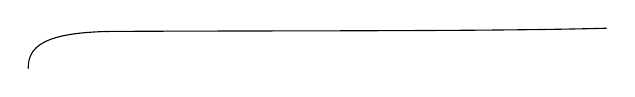
\begin{tikzpicture}[x=.02cm,y=.01cm,line cap=round]\draw[thin] (0,0)..controls(0,26)and(8,47)..(57,47)..controls(162,48)and(294,47)..(367,51);\end{tikzpicture}\end{tabular}}, et cette dernière est de carré nul grâce à la condition $\gamma$.

\margin{dégager un lemme circonstancié\,\ldots.
\figure{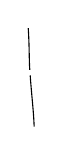
\begin{tikzpicture}[x=1cm,y=1cm]
\draw[thin] (0,1.25) .. controls (0.015,1.05) and (0.01,0.84) .. (0.02,0.72);
\draw[thin] (0.025,0.65) .. controls (0.04,0.43) and (0.07,0.18) .. (0.075,0);
\end{tikzpicture}}}

3.\quad \deleted{Algèbre} \unsure{\deleted{de}|de} \uline{Anneau de Lie} \uline{associé à un complexe de De Rha\unsure{m}}

Soit $\mathfrak g=\underline{\mathrm{Hom}}(\Omega,\underline O_{X_0})$, c'est un ind-module quasi-ch. sur $X_0$, qu'on identifie à un Module qu. coh.

Ceci definit, si $X,Y$ sont des sections de $\mathfrak g$ \deleted{\unsure{sur}} sur un $U$
\[
[X,Y]\deleted{(\omega)}\in\Gamma(U,\mathfrak g)\qquad\text{avec}
\]
\[
\begin{aligned}
(x)\qquad &\left\langle\underset{\substack{\rotatebox{-90}{$\in$}\\\Gamma(U,\Omega)}}{\omega},[X,Y]\right\rangle
\deleted{\unsure{(\omega)}}=-\langle\unsure{:}\delta\omega,X\wedge Y\rangle
\unsure{\deleted{-}+|+|\deleted{+}-}\Theta_X\langle\omega,Y\rangle
\overset{\inserted{-}}{\deleted{+}}\Theta_Y\langle\omega,X\rangle
\end{aligned}
\]
où l'action $X\mapsto\Theta_X$ de $\mathfrak g$ sur $\underline O_{X_0}$ \inserted{\begin{tabular}[b]{@{}l@{}}(par dérivations)\\[-1.2ex]
\begin{tikzpicture}[x=1cm,y=1cm]
\draw[thin] (0,-0.2) .. controls (0,0.08) and (0.12,0.15) .. (0.35,0.15) -- (2.7,0.15) .. controls (2.95,0.15) and (3,0.18) .. (3,0.3);
\end{tikzpicture}
\end{tabular}} est definie par
\[
\Theta_X(f)=\langle\delta f,X\rangle,\qquad
[\,\text{NB}\quad\vcenter{\hbox{\sbox0{$\displaystyle \Theta_{gX}=g\,\unsure{\Theta|\deleted{=}\Theta|\deleted{\Theta}=}_X$}\rlap{\raisebox{\dimexpr-\dp0-.4em\relax}{\resizebox{\dimexpr\wd0+.8em\relax}{\dimexpr\ht0+\dp0+.8em\relax}{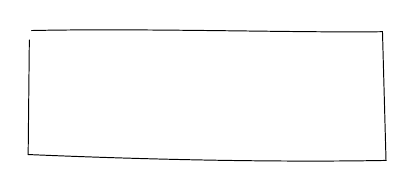
\begin{tikzpicture}[x=.15mm,y=.15mm,line cap=round]\draw[line width=.35pt] (3,110)..controls(100,112)and(232,108)..(300,109)--(303,0)..controls(190,-2)and(70,2)..(0,5)--(1,102);\end{tikzpicture}}}}\hspace{.4em}\usebox0\hspace{.4em}}}\,]\quad\text{resulte de rien}
\]
\[
\text{(resulte de }\unsure{\alpha)}\text{)}\quad
\vcenter{\hbox{\sbox0{$\displaystyle \Theta_X(fg)=\unsure{\Theta|\deleted{=}\Theta|\deleted{\Theta}=}_X(f)g+f\Theta_{\unsure{X|\deleted{g}X|\deleted{X}g}}(g)$}\rlap{\raisebox{\dimexpr-\dp0-.4em\relax}{\resizebox{\dimexpr\wd0+.8em\relax}{\dimexpr\ht0+\dp0+.8em\relax}{\begin{tikzpicture}[x=.15mm,y=.15mm,line cap=round]\draw[line width=.3pt] (0,53)..controls(2,41)and(2,25)..(3,11)..controls(120,4)and(330,2)..(455,0); \draw[line width=.3pt] (311,76)..controls(360,75)and(420,70)..(455,72)..controls(459,72)and(460,63)..(459,59);\end{tikzpicture}}}}\hspace{.4em}\usebox0\hspace{.4em}}}
\]
On constate \inserted{\begin{tabular}[b]{@{}l@{}}grâce à $\alpha)$ et $\beta)$\\[-1.2ex]
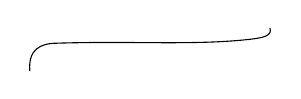
\begin{tikzpicture}[x=1cm,y=1cm]
\draw[thin] (0,-0.2) .. controls (-0.02,0.07) and (0.13,0.15) .. (0.35,0.15) .. controls (1.3,0.18) and (2.1,0.12) .. (2.8,0.2) .. controls (2.98,0.22) and (3.08,0.25) .. (3.05,0.34);
\end{tikzpicture}
\end{tabular}} que le deuxi\unsure{è|e}m\unsure{e|.} mb de $(x)$ est bien \uline{$\underline O_{X_0}$-linéaire} en $\omega$, donc definit une section $X\wedge Y$.

De plus, on aura, utilisant $\unsure{\gamma)}$
\[
\begin{aligned}
(xx)\qquad &\deleted{\unsure{[X,Y]}}\quad
\vcenter{\hbox{\sbox0{$\displaystyle \Theta_{[X,Y]}=[\Theta_X,\Theta_Y]$}\rlap{\raisebox{\dimexpr-\dp0-.4em\relax}{\resizebox{\dimexpr\wd0+.8em\relax}{\dimexpr\ht0+\dp0+.8em\relax}{\begin{tikzpicture}[x=.15mm,y=.15mm,line cap=round]\draw[line width=.35pt] (0,124)..controls(0,85)and(3,25)..(7,0)..controls(180,8)and(425,13)..(530,26)--(526,143); \draw[line width=.3pt] (10,137)..controls(130,133)and(430,177)..(525,160);\end{tikzpicture}}}}\hspace{.4em}\usebox0\hspace{.4em}}}
\overset{\mathrm{df}\unsure{\mathrm{n}}}{=}
\Theta_X\Theta_{\unsure{Y|\deleted{X}Y|\deleted{Y}X}}\deleted{f}-\Theta_{\unsure{Y|\deleted{X}Y|\deleted{Y}X}}\Theta_X
\end{aligned}
\]
\deleted{[Si on veut l'autre definition}

[Sans $\gamma$, la \deleted{valeur des} difference des deux mbs sur $f$ est $-\langle\delta\delta f,X\wedge Y\rangle$ ; donc si $\Omega$ loc libre, la condition $\delta_1\delta_0=0$ est né\uline{cessai}re pour qu'on ait $(xx)$]. Ceci vérifie aussi la loi de Lie
\margin{\hbox{\sbox0{\scriptsize\unsure{trivial|finir}}\rlap{\raisebox{-1.7em}{\resizebox{\dimexpr\wd0+1em\relax}{3.5em}{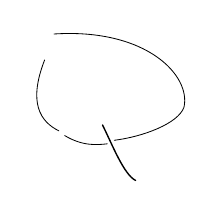
\begin{tikzpicture}[x=.15mm,y=.15mm,line cap=round]\draw[line width=.3pt] (16,124)..controls(94,129)and(132,89)..(126,62)..controls(121,48)and(91,37)..(67,34); \draw[line width=.3pt] (8,102)..controls(-6,66)and(4,50)..(20,42); \draw[line width=.3pt] (25,38)..controls(40,29)and(52,30)..(61,31); \draw[line width=.5pt] (57,47)..controls(65,31)and(75,5)..(85,0);\end{tikzpicture}}}}\hspace{.5em}\usebox0\hspace{.5em}}}
\[
\vcenter{\hbox{\sbox0{$\displaystyle [X,X]=0$}\rlap{\raisebox{\dimexpr-\dp0-.4em\relax}{\resizebox{\dimexpr\wd0+.8em\relax}{\dimexpr\ht0+\dp0+.8em\relax}{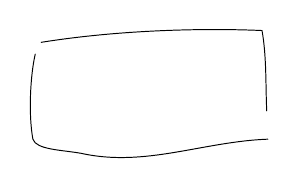
\begin{tikzpicture}[x=.15mm,y=.15mm,line cap=round]\draw[line width=.35pt] (8,94)..controls(77,105)and(149,106)..(195,104)..controls(199,82)and(198,56)..(199,36); \draw[line width=.35pt] (200,12)..controls(145,10)and(96,-12)..(42,0)..controls(25,3)and(4,3)..(1,12)..controls(-3,34)and(-1,67)..(3,84);\end{tikzpicture}}}}\hspace{.4em}\usebox0\hspace{.4em}}}\unsure{f,|\gamma)|\lambda)}\qquad
\vcenter{\hbox{\sbox0{$\displaystyle [[X,Y],Z]+[[Y,Z],X]+[[Z,X],Y]=0$}\rlap{\raisebox{\dimexpr-\dp0-.4em\relax}{\resizebox{\dimexpr\wd0+.8em\relax}{\dimexpr\ht0+\dp0+.8em\relax}{\begin{tikzpicture}[x=.15mm,y=.15mm,line cap=round]\draw[line width=.3pt] (0,108)..controls(0,63)and(1,25)..(4,5); \draw[line width=.3pt] (24,13)..controls(58,2)and(156,13)..(650,22)..controls(830,30)and(1020,20)..(1110,21)--(1115,45); \draw[line width=.3pt] (8,128)..controls(90,128)and(180,158)..(600,157)..controls(840,162)and(1060,159)..(1110,158)..controls(1118,156)and(1119,102)..(1128,59)..controls(1130,54)and(1126,50)..(1121,50);\end{tikzpicture}}}}\hspace{.4em}\usebox0\hspace{.4em}}}
\]
}
\margin{23}

